\section{Search for a Kinematic Edge}
\label{sec:fit}

Any new physics process which produces leptons via a cascade decay chain will lead to final states
containing same-flavor (SF) $ee$ or $\mu\mu$ lepton pairs only, provided that lepton flavor
is conserved. In contrast, for the dominant background \ttbar\ as well as other
SM processes such as $W^+W^-$ and $\mathrm{DY}\to\tau^+\tau^-$, the 2 lepton flavors are uncorrelated,
and the rates for SF and opposite-flavor (OF) $e\mu$ lepton pairs are therefore the same.
Hence we can search for new physics in the SF final state, and model the backgrounds
using events in the OF final state. 

In Sec.~\ref{sec:datadriven} we search for an excess of
events with SF with respect to OF lepton pairs, accompanied by large \met\ and \Ht. 
In this section, we search for a kinematic edge in the dilepton mass distribution for same-flavor
events. This edge is a characteristic feature of, for example, SUSY scenarios in which
the opposite-sign leptons are produced via the decay $\chi_2^0 \to \chi_1^0 \ell^+\ell^-$.
The \ttbar\ background shape is extracted from events with OF lepton pairs, and we perform
a fit to the dilepton mass distribution in events with SF lepton pairs.

Since we wish to examine the dilepton mass over the full range, in this section only we do not
veto SF events in the $Z$ mass region. This increases the DY contribution, and the \MET\ requirement 
is increased to \MET $>$ 100 GeV to compensate.
We search for the kinematic edge in 2 regions.  The first is a control region defined
as 100 $<$ \Ht\ $<$ 300 GeV, which is dominated by the \ttbar\ background; we use 
this region to validate our fit methodology and verify that a signal yield consistent with 0 
is obtained. We then proceed to search for a kinematic edge in the signal region defined as 
\Ht\ $>$ 300 GeV. Since we do not observe a kinematic edge in this region, we perform a 
fit to the dilepton mass distribution assuming an example signal shape from the LM1 scenario.

The contributions from fake leptons are treated as negligible, since they are measured
to be roughly 1\% of the total background using the data-driven fake rate technique.
The residual DY contribution in the signal region is extrapolated from a control region at lower \Ht,
and is found to be negligible.
 
The background as a function of the invariant mass $\mll$ is described by:

\begin{equation}
B(\mll) = \mll^a e^{-b \mll},
\end{equation}
where $a\approx1.5$ describes the rising edge and $b\approx0.003$
dominates the long exponential tail on the right hand side of the 
shape. The extracted shape compared to the dilepton mass distribution in the control region
for events containing OF lepton pairs is shown in Fig.~\ref{fig:dilmass} (upper-right).

For a potential signal, we use an edge model for two subsequent two-body decays, 
which comprises a triangular shape convoluted with a gaussian,
according to:

\begin{equation}
T(\mll) = \frac{1}{\sqrt{2\pi}\sigma}\int_0^{M_{cut}} dy~y e^{\frac{(-(\mll-y)^2}{2\sigma^2}},
\end{equation}

where the resolution parameters for electrons $\sigma_{ee}$ and muons $\sigma_{\mu\mu}$ are constrained 
based on simulation.

\begin{figure}[hbt]
\begin{center}
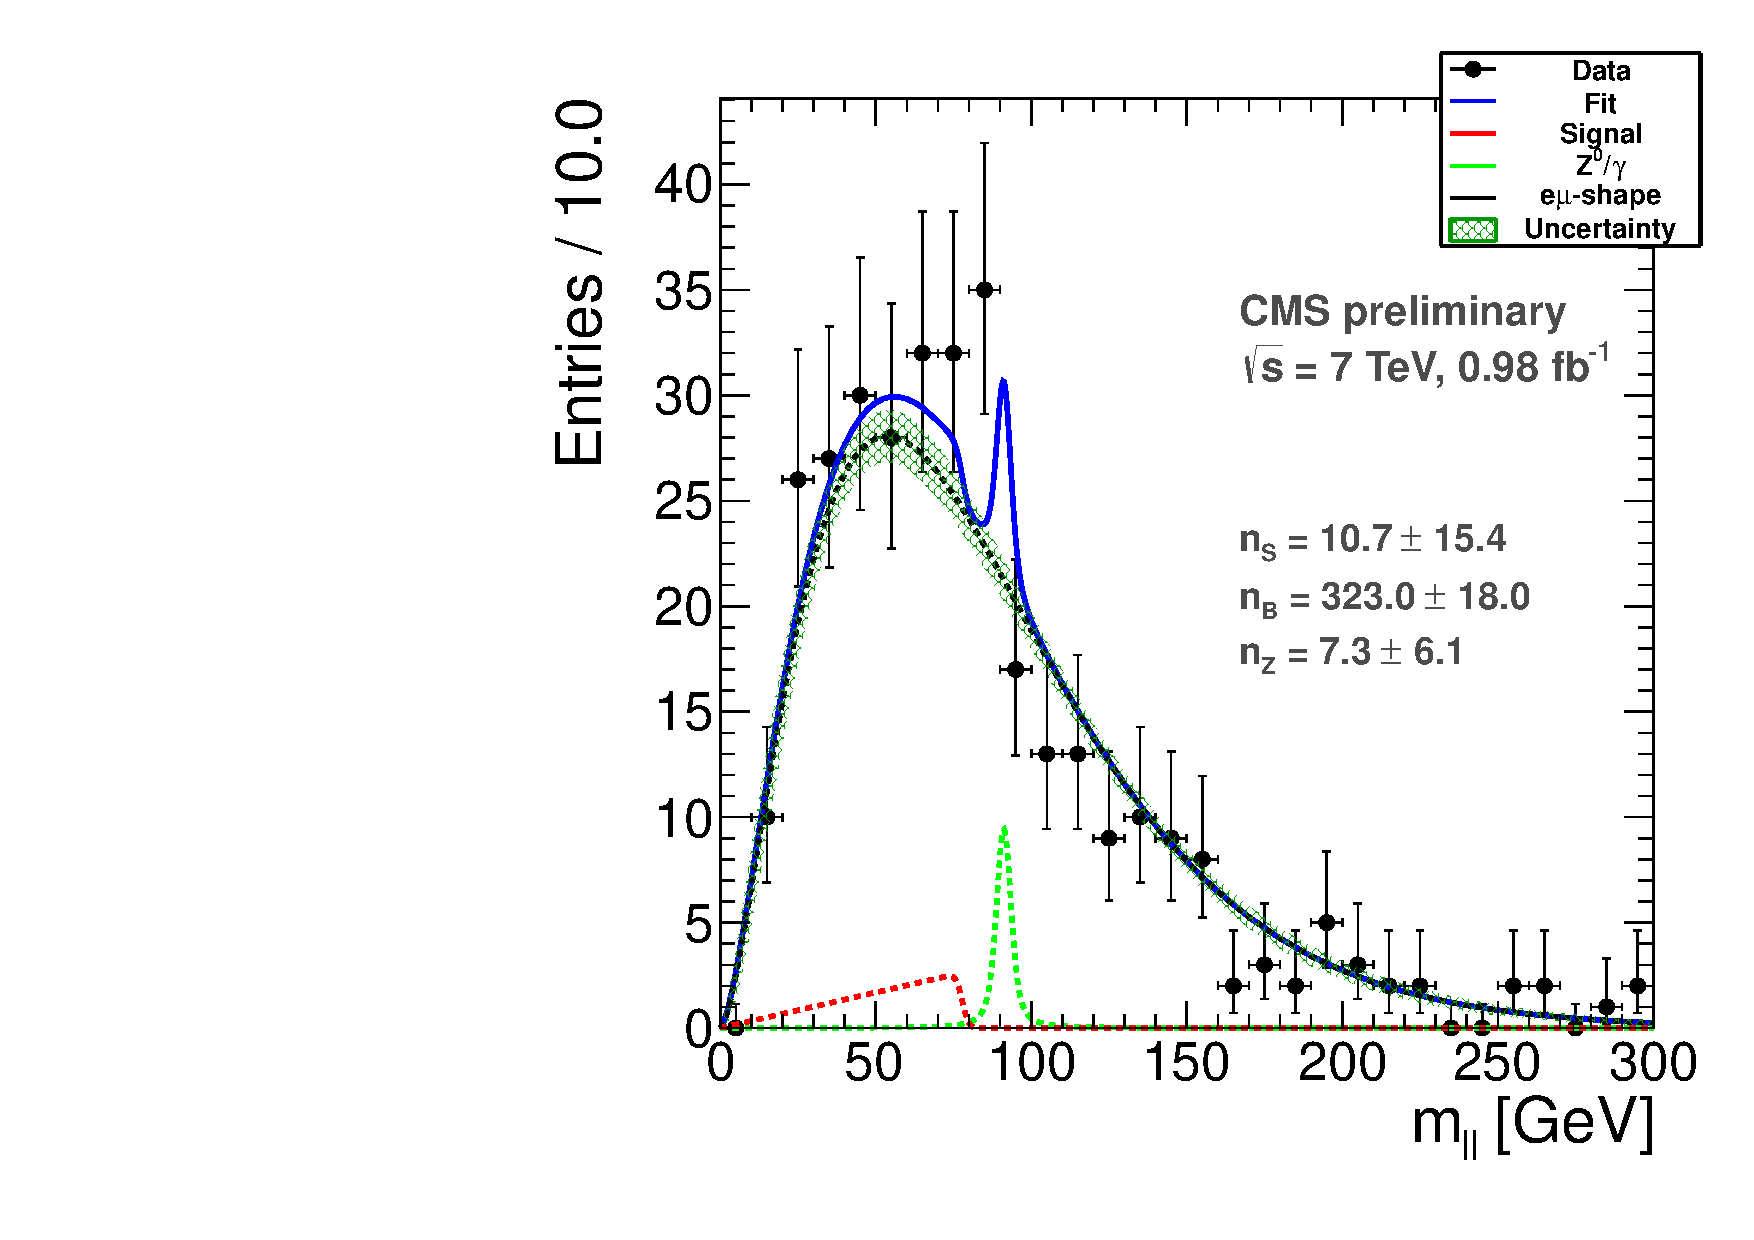
\includegraphics[width=0.48\linewidth]{plots_final/fit2011_Control_Data.pdf}
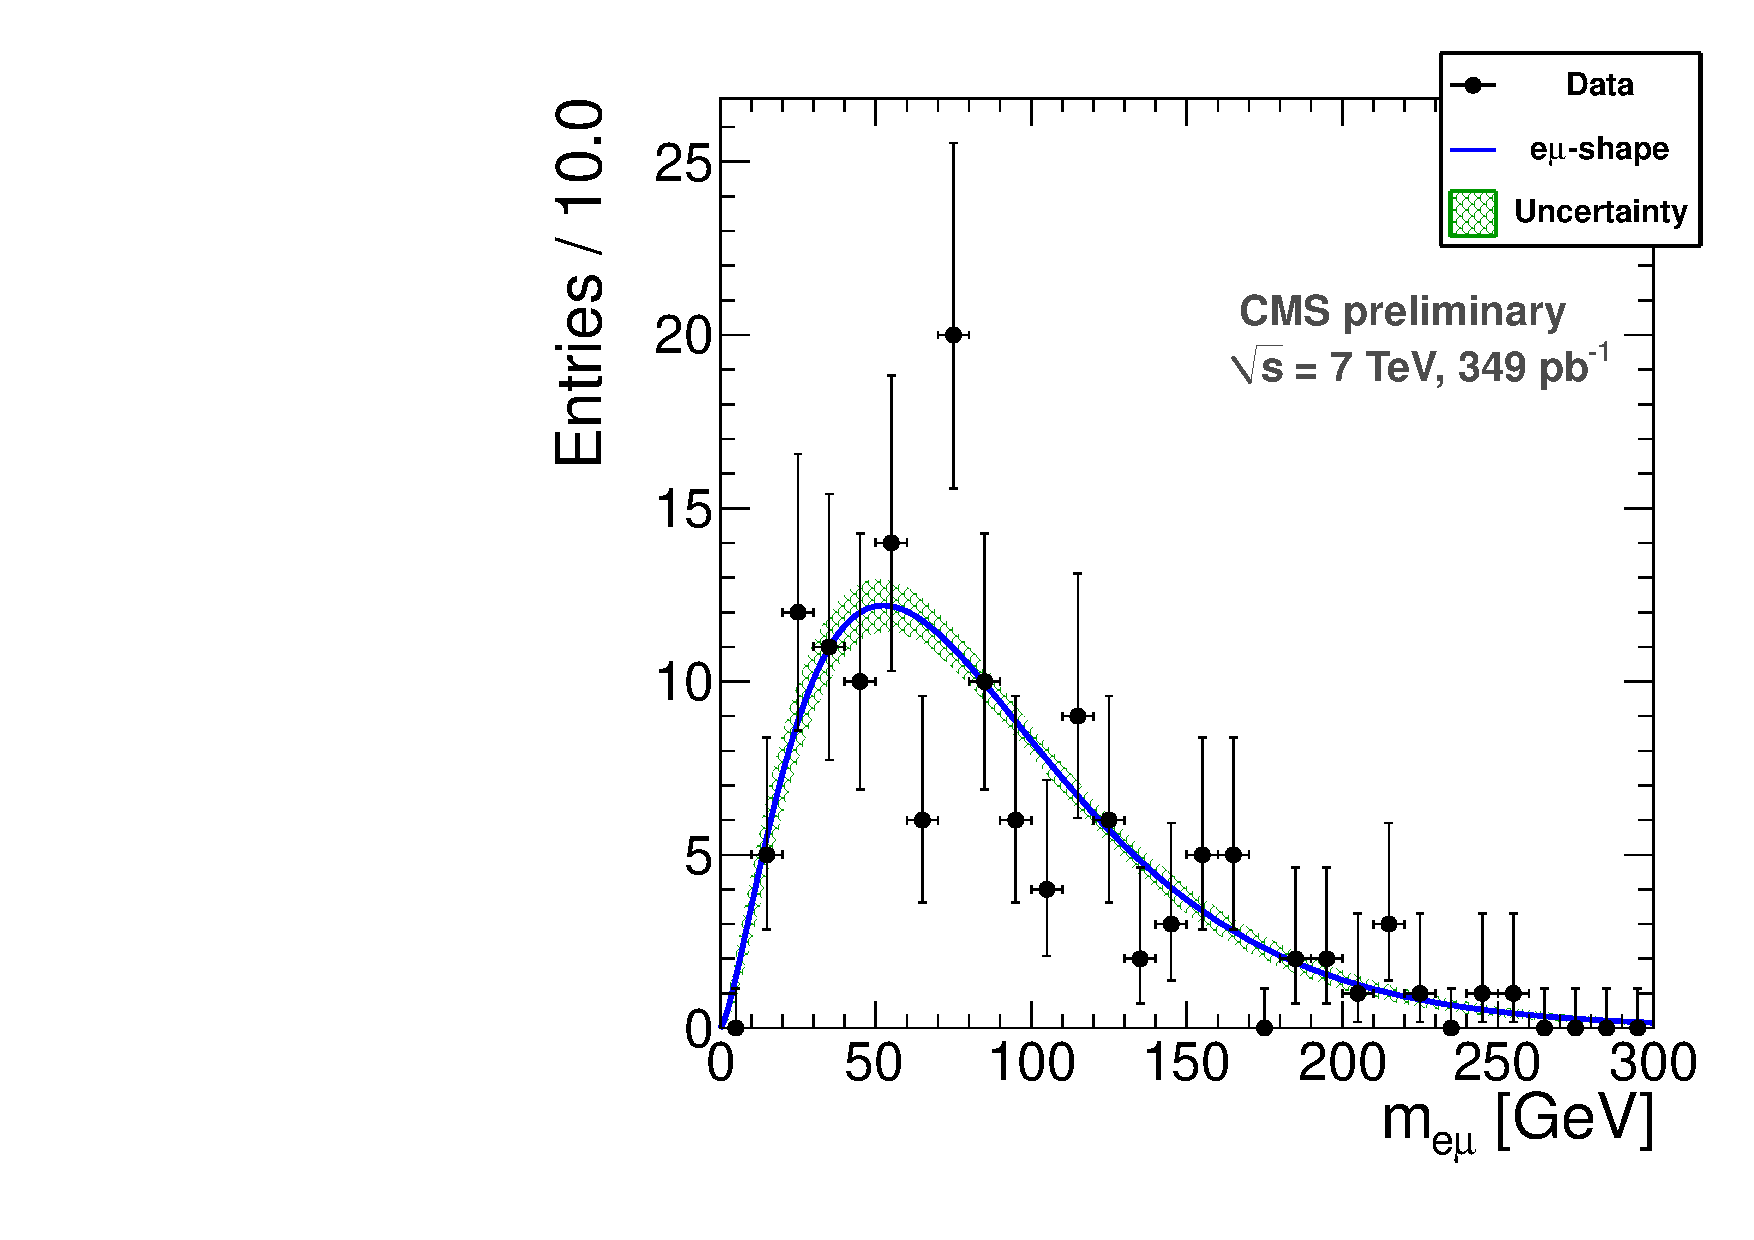
\includegraphics[width=0.48\linewidth]{plots_final/fit2011OFOS_Control_Data.pdf}
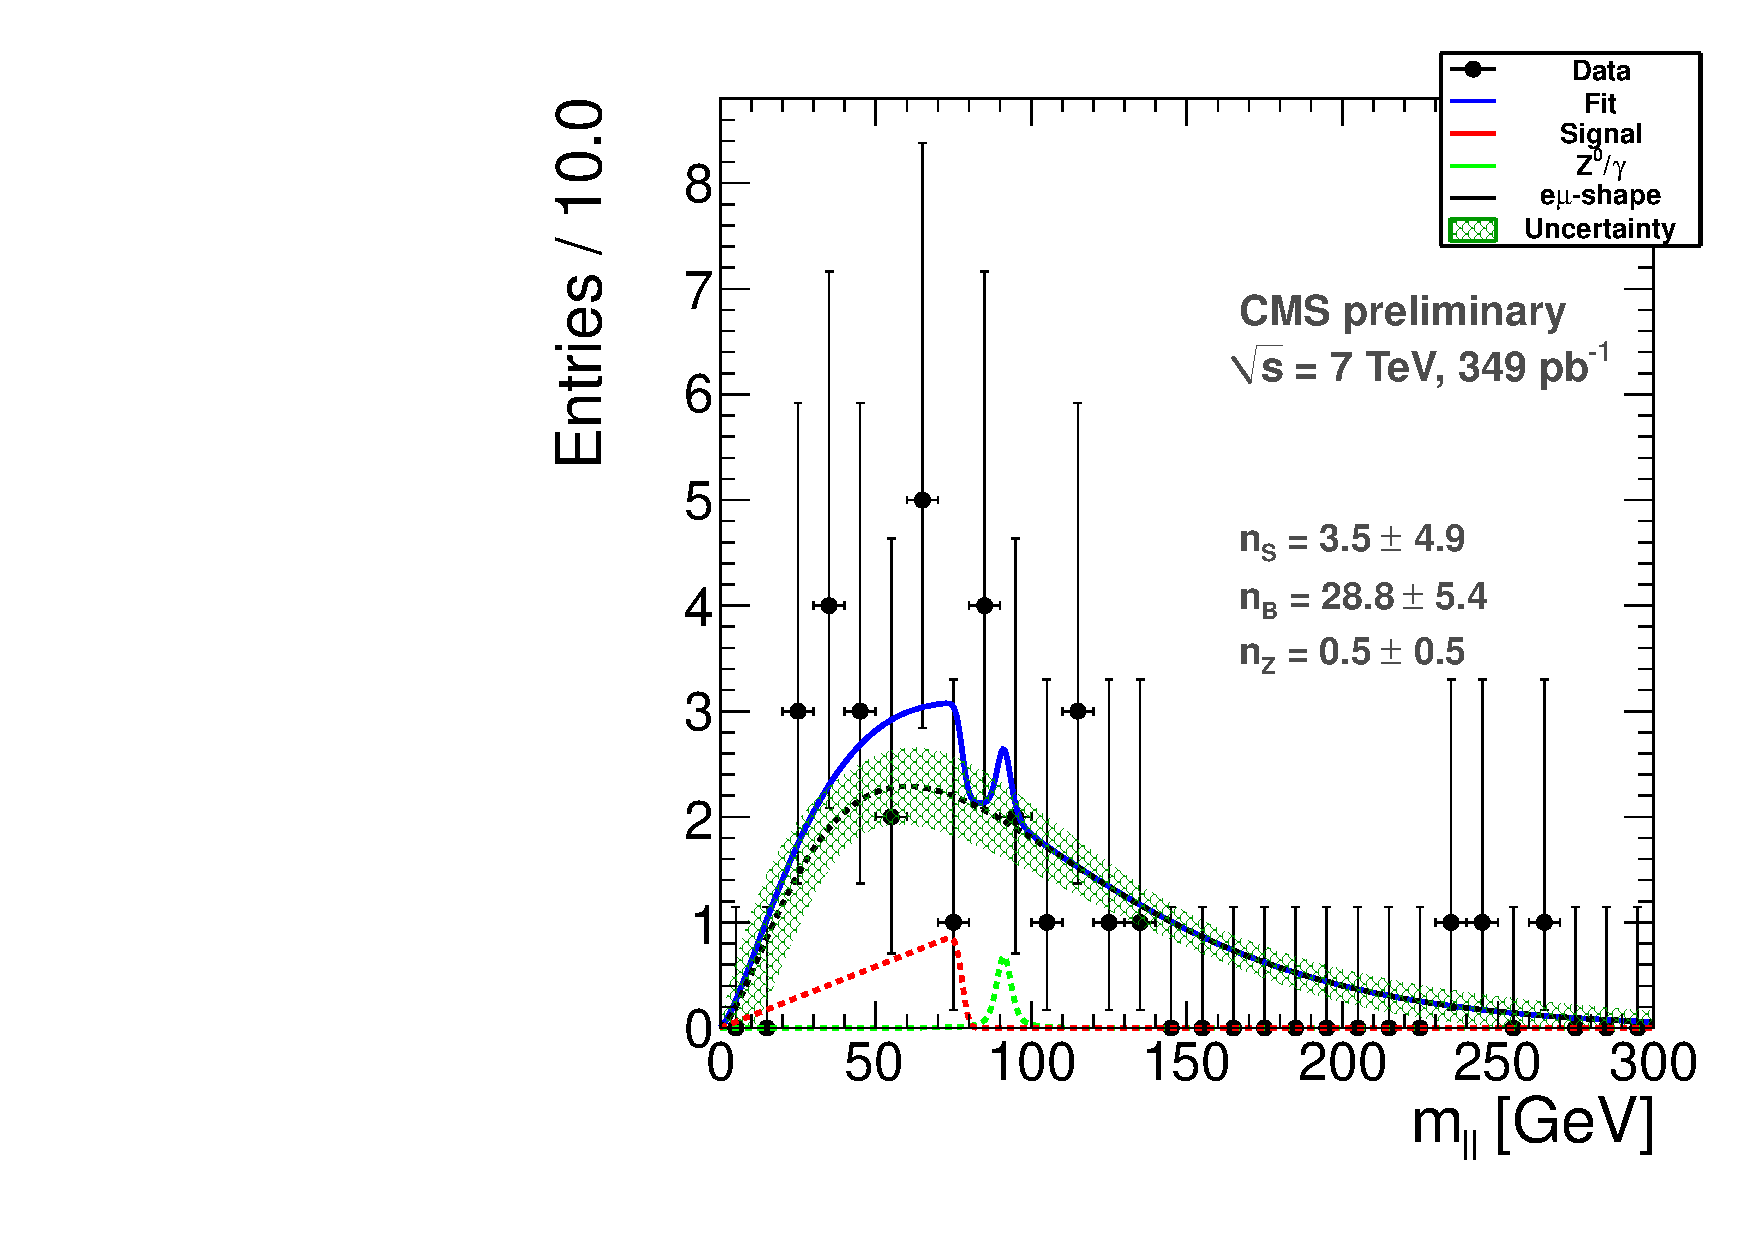
\includegraphics[width=0.48\linewidth]{plots_final/fit2011_Signal_Data.pdf}
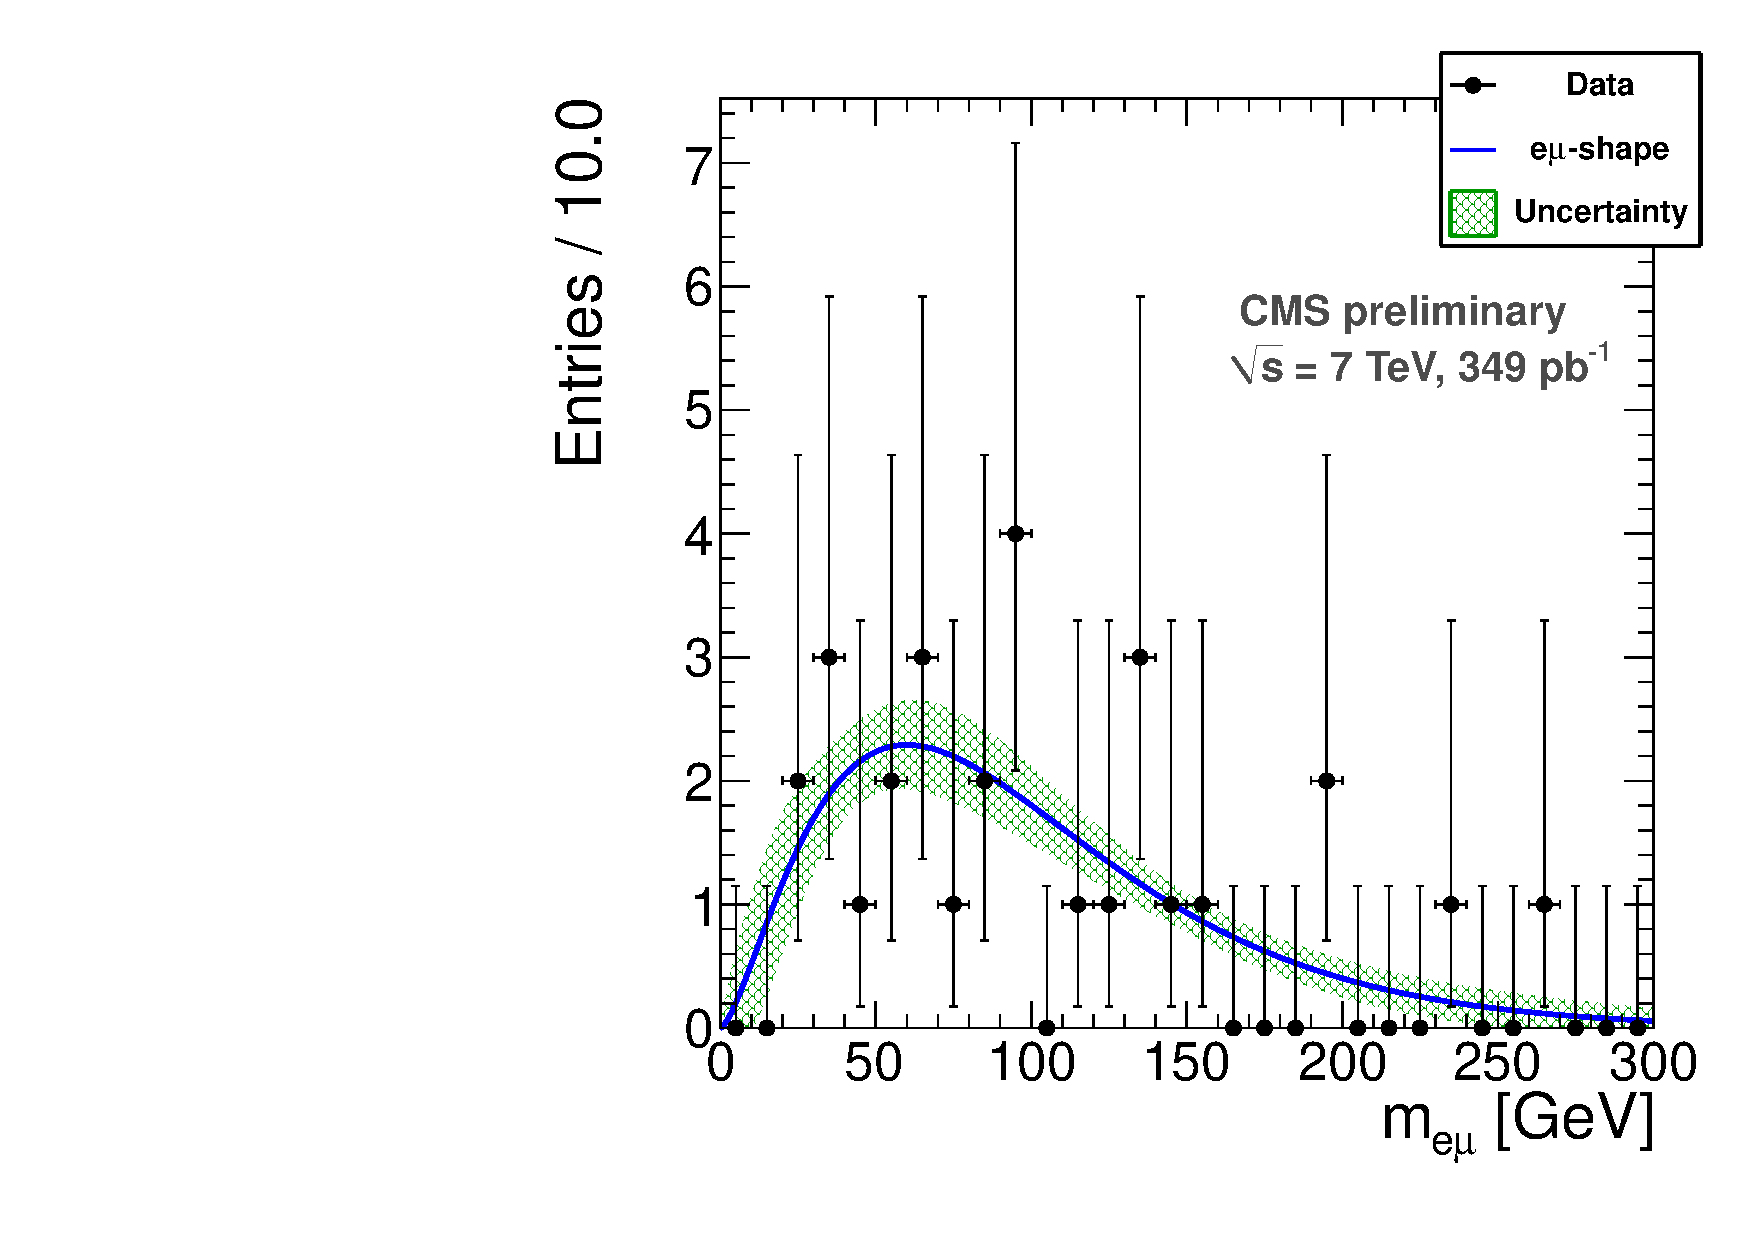
\includegraphics[width=0.48\linewidth]{plots_final/fit2011OFOS_Signal_Data.pdf}
\caption{\label{fig:dilmass}\protect 
Results of the maximum likelihood fit to the dilepton mass distribution for events containing 
$ee$ and $\mu\mu$ lepton pairs (left) and $e\mu$ lepton pairs (right) in the control
region defined as 100 $<$ \Ht\ $<$ 300~GeV, \MET\ $>$ 100 GeV (upper) and the signal region
\Ht\ $>$ 300~GeV, \MET\ $>$ 100 GeV (lower). In the extended fit the number of
signal $n_{S}$, $Z$ $n_Z$ and \ttbar\ $n_B$ events is extracted as well.
}
\end{center}
\end{figure}

The position of the kinematic edge $M_{cut}$ is fixed based on the generator level
information for the signal model which is tested; for example, for LM1 
$M_{cut} = 77.8$~GeV. Finally, the $Z$ contribution is modelled by a Breit-Wigner 
convoluted with a Gaussian (with fixed $Z$ mass and width). 

We perform a simultaneous, extended, unbinned maximum 
likelihood (ML) fit to the distribution of dilepton mass for events containing $ee$, $\mu\mu$ 
(signal, $Z$ and background model)
and $e\mu$ pairs (background model only). 
The shape of the \ttbar\ background is assumed to be common in all categories.
The fit is performed separately for events with $ee$, $\mu\mu$ and $e\mu$ lepton pairs,
and the yields of signal $n_S$, $Z$ $n_Z$ and background $n_B$ 
in these three categories are constrained using the ratio of muon to electron selection efficiencies
$R_{\mu e} = 1.13 \pm 0.05$. This quantity is evaluated as the square root of the ratio of the number of 
$Z \to \mu^+\mu^-$ to $Z \to e^+e^-$ events in data, in the mass range 76-106 GeV with no jets or 
\met\ requirements. 

We perform the fit in the control region 100 $<$ \Ht\ $<$ 300 GeV, in
which the \ttbar\ background, $Z$ background, and LM1 signal yields are allowed to vary in the fit. 
The extracted signal yield, constrained to be positive, is $n_S = 0.0 \pm 7.3$, 
consistent with the background only 
hypothesis, as displayed in Fig.~\ref{fig:dilmass} (upper-left). 
The extracted $Z$ yield is $n_Z = 5.2 \pm 4.2$, which is 
used to constrain the $Z$ yield in the signal region. 

Next, we perform the fit in the signal region \Ht\ $>$ 300 GeV. The \ttbar\ shape
overlaid with OF events is shown in Fig.~\ref{fig:dilmass} (lower-right). We
constrain the $Z$ yield in this region using an extrapolation in \Ht\ from the 
control region 100 $<$ \Ht\ $<$ 300 GeV. The $Z$ yield in the control region is
multiplied by a scale factor derived from $Z$ events in data with no requirement
on \MET, which quantifies the fraction of $Z$ events with \Ht\ $>$ 100 GeV which 
satisfy \Ht\ $>$ 300 GeV. Using this procedure we derive an upper limit on the
$Z$ yield in the signal region of $n_Z < 0.5$, which we use to constrain the
$Z$ yield in the ML fit. The extracted signal yield is $n_S = 3.5 \pm 4.9$,
which is consistent with the background only hypothesis,
as shown in Fig.~\ref{fig:dilmass} (lower-left). The expected LM1
yield in this region is $23\pm2 $ events.
